\documentclass[Lecture.tex]{subfiles}
\begin{document}
\section{2.3: Summarizing One or Two Categorical Variables}
\begin{frame}{Definition}
  \begin{defn}
  In general, the {\it distribution} of a variable describes how often the possible responses occur.
    \begin{itemize}
    \item<1->
      A {\it frequency distribution} for a categorical variable is a listing of all categories along with their frequencies (counts).
    \item<2->
      A {\it relative frequency distribution} is a listing of all categories along with their relative frequencies (given as proportions or percentages).
    \end{itemize}
  \end{defn}
\end{frame}




\begin{frame}{Example}
A survey of 479 children found that those who had slept with a nightlight or in a fully lit room before the age of 2 had a higher incidence of nearsightedness (myopia) later in childhood ({\it Sacramento Bee}, May 13, 1999, pp. A1, A18).
\begin{center}
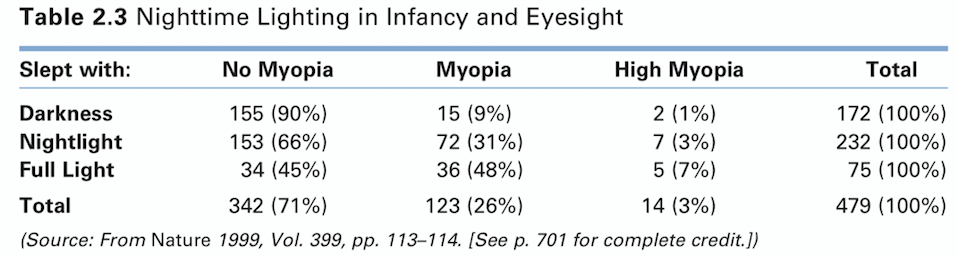
\includegraphics[scale=.3]{myopia}
\end{center}
\end{frame}

\begin{frame}{Visual Summaries for Categorical Variables}
\begin{center}
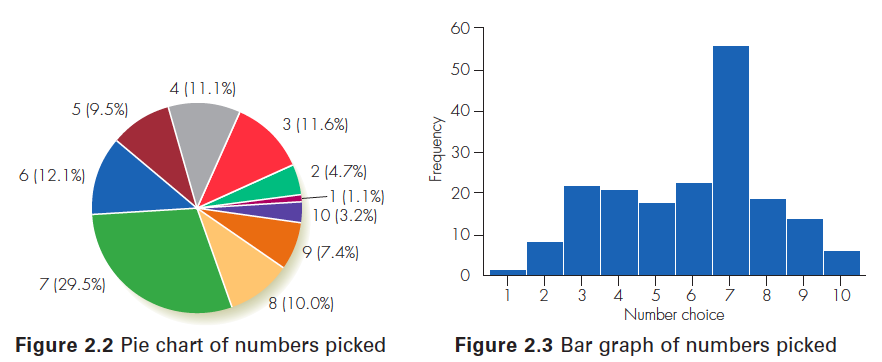
\includegraphics[scale=.3]{charts}
\end{center}
\end{frame}

\begin{frame}{Visual Summaries for Categorical Variables}
\begin{center}
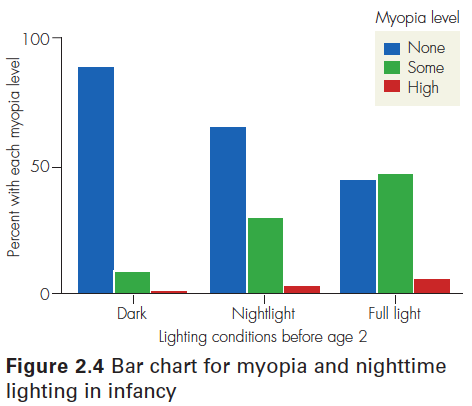
\includegraphics[scale=.4]{charts2}
\end{center}
\end{frame}

\end{document}